% 我们工作的'理论基础'
% 放上定理即可
\begin{frame}{Analysis of Online-FAST}
\begin{block}{Theorem 1: Fairness Degree Converges to Zero}
Given the arriving probability $A$ for the user set, the sum of Top-N Fairness Degree of all the users in each round will approach to zero (i.e.  $\lim_{T \rightarrow \infty}\sum_{u_{i} \in U} F_{i}^{T}=0$) if and only if the users share a same arriving probability.
\label{thm1}
\end{block}
% ps: Proof of Theorem 1 can be checked in our paper.\\


\begin{figure}[H]
  \centering
  \subfigure{
    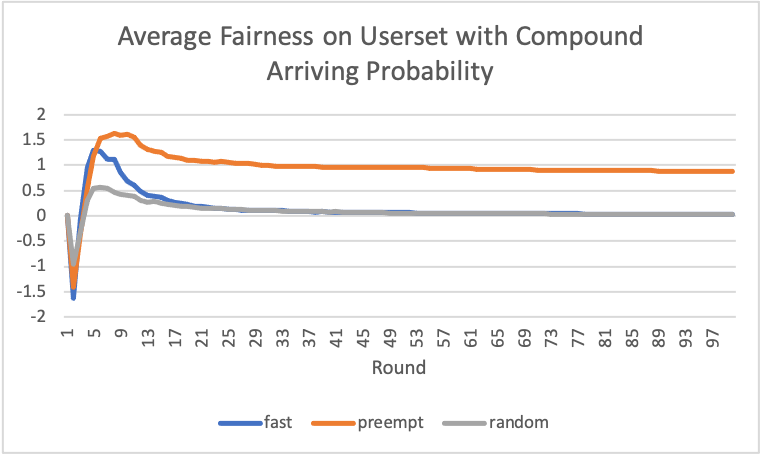
\includegraphics[scale=0.21]{img/thr1.png}}
  \hspace{0.1in} % 两图片之间的距离
  \subfigure{
    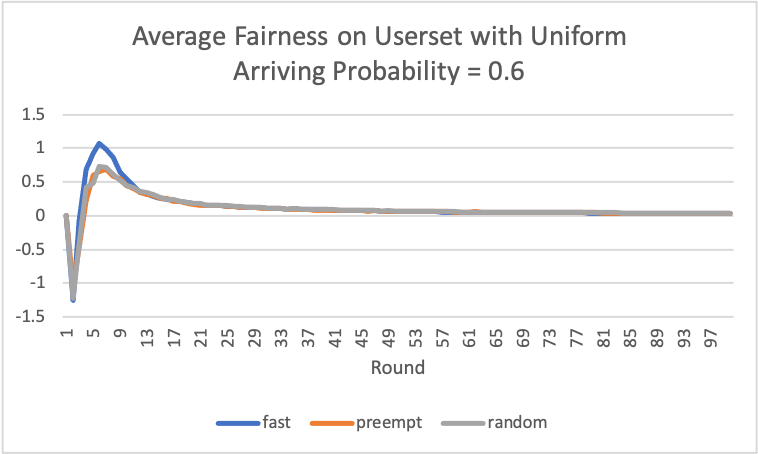
\includegraphics[scale=0.21]{img/thr2.png}}
  \caption{An intuitive interpretation of Theorem 1}
\end{figure}

\end{frame}

\begin{frame}{Analysis of Online-FAST}
%第二个定理依赖了一些直觉上的推论和随机性的假设
Based on the result of Theorem 1,
we have the following claim:
\begin{block}{Claim: Variance Convergence}
For a group of users with the same arriving probability, assume the arrival of them are uniformly distributed. The variance among the Top-N fairness of them $D\left(F_{i}^{T}\right)$ converges with the recommended round $T$.
\end{block}
\begin{enumerate}
    \item This claim is based on intuitive inference and assumption of randomness;
    \item Its validness and versatility can be checked with experiments in real cases.
\end{enumerate}
\end{frame}


